% LaTeX Source file for Cytoscape Manual Chinese Edition
% File name: ch01.tex
% Author: Chen Gang (chen.gang1983@gmail)
% Date: March 3th, 2009
% License: GPL 3.0 or later


Cytoscape~是一个Java程序,能在~Linux~、~Windows~和~Mac OS X~上运行。对于其他能安装Java 5的操作系统平台,比如以Solaris和FreeBSD为代表的UNIX,Cytoscape也能运行,但官方并对此提供支持。

\section{系统要求}
	Cytoscape~对系统的具体要求取决于所加载、查看和操作的网络的大小。

	\begin{table}[htbp]
	\label{tabel:2}
	\centering
	\begin{tabular}{|l|l|l|}
	\hline
	 & 小型网络查看 & 大型网络分析和查看 \\
	\hline
	处理器 & 1GHz & 尽可能的快\\
	\hline
	内存   & 512MB & 2GB以上 \\
	\hline
	显卡   & 板载集成显卡 & 高端独立显卡 \\
	\hline
	显示器 & XGA($1024 \times 768$) & 高分辨率或双显示器 \\
	\hline
	\end{tabular}
	\caption{}
	\end{table}

\section{入门}
	\subsection{安装~Java}
		如果计算机上还没有安装~Java,那么首先要下载并安装~Java SE 5~或~6~。\textbf{Cytoscape~从2.5版开始就不能在~Java 1.4~上运行。必须安装~Java SE 5~或~6~!!!}
		Java SE 5~和~Java SE 6可以从这里下载:
		\begin{itemize}
		\item \href{http://java.sun.com/javase/downloads/index_jdk5.jsp}{Java SE 5}
		\item \href{http://java.sun.com/javase/downloads/index.jsp}{Java SE 6}
		\end{itemize}
	
		一般情况下,Java SE 6~的运行速度要快一些。所以,如果您的计算机兼容~Java SE 6~的话,请尽量使用~Java SE 6。

	\subsection{安装~Cytoscape}
		Cytoscape~供下载的版本很多,安装方法也不尽相同。所有的版本都可以从~http://cytoscape.org~网站下载。
		
		\begin{itemize}
		\item Windows、Mac OS以及Linux平台上的自动安装包
		\item 压缩发行版
		\item 从源代码编译
		\item 从Subversion源中提取最新版的软件
		\end{itemize}

		Cytoscape的安装目录(无论是什么平台)中包含表~\ref{table:3}~中的文件。

		\begin{table}[!h]
		\begin{tabular}{|l|l|}
			\hline
			文件 & 描述 \\
			\hline
			cytoscape.jar & Cytoscape~的主程序(~Java~压缩包)。\\
			\hline
			\multirow{2}{*}{cytoscape.sh} & 从命令行运行~Cytoscape~的脚本(用于~Linux~和~\\&Mac OS X~)。\\
			\hline
			cytoscape.bat & 运行Cytoscape的脚本(用于~Windows~)。\\
			\hline
			LICENSE.txt/html & Cytoscape GNU LGPL~授权。\\
			\hline
			lib/ & Cytoscape运行所需的jar库。\\
			\hline
			docs/ & 各种格式的用户手册。也就是你正在阅读的东西。\\
			\hline
			plugins/ & jar格式的Cytoscape插件。\\
			\hline
			sampleData/ & \\
			\hline
				& galFiltered.gml -- 分子相互作用网络数据示例$^*$。\\
			\hline
				& galFiltered.sif -- Simple Interaction~格式的同一个网络$^*$\\
			\hline
				& galExpData.pvals -- 基因表达矩阵文件示例$^*$。\\
			\hline
				\multirow{2}{*}{} & galFilteredAttrTable.xls -- 微软~Excel~格式的节点属性\\ & 文件示例。\\
			\hline
				\multirow{2}{*}{} & galFiltered.sif -- 用上面的数据库和多个注释数据库创建\\ & 的会话示例$^*$。\\
			\hline
				\multirow{2}{*}{} & BINDyeast.sif -- BIND数据库中酵母的蛋白质相互作用\\ & 网络,2006年12月$^{**}$。\\
			\hline
				\multirow{2}{*}{} & BINDhuman.sif -- BIND数据库中人类的蛋白质相互作\\ & 用网络,2006年12月$^{**}$。\\
			\hline
				& yeastHighQuality -- 分子生物相互作用的示例文件$^{***}$。\\
			\hline
				\multirow{2}{*}{} & interactome\_{}merged\_{}networkTable.gz -- 制表符分割格\\ & 式的人类相互作用网络$^{****}$。\\
			\hline
				& sampleStyle.props -- 附加的~Visual Sytle~示例。\\
			\hline
		\end{tabular}
		\caption{$^*$ 来自~Ideker er al, Science 292:929 (2001); $^{**}$ 来自~http://www.blueprint.org/bind/bind\_{}downloads.html; $^{***}$ 来自~Mering et al, Nature, 417:399 (2002) Lee et al, Science 298:799 (2002);$^{****}$来自~Cytoscape~教程网页。原始数据可以从~http://cytoscape.org/cgi-bin/moin.cgi/Data\_{}Sets/上由Andrew Garrow、Yeyejide Adeleye和Guy Warner(Unilever, Safety and Enviromental Assurance Center)创建的“A merged human interactome”中下载。 }
		\label{table:3}
		\end{table}

	\subsection{启动程序}
		双击安装程序创建的图标,或是在命令行中运行~cytoscape.sh(Linux或Mac OS X),也可以双击~cytoscape.bat(Windows)~就能启动~Cytoscape。还可以在命令行中将这个jar文件以命令行参数的形式传递给命令~java -Xmx512M -jar cytoscape.jar -p plugins~。~-Xmx512M~标志是告诉~java~给~Cytoscape~分配较多的内存,~-p plugins~则是告诉~Cytoscape~加载~plugins~目录中所有的插件。插件对于~Cytoscape~是非常重要的,诸如布局(layout)、过滤器(filter)和属性浏览器之类的功能都是由插件提供的。关于命令行参数的详细信息请阅读\textit{命令行参数}一章。在~Windows~中,只需要双击~jar~文件就能启动~Cytoscape。不过,这样就不能使用命令行参数了(比如制定插件目录的位置)。

		成功地启动~Cytoscape后,就会看到如图~\ref{fig:1.1}~所示的窗口(图~\ref{fig:1.1}~来自Mac OS 10.4)。

		\begin{figure}[h]
			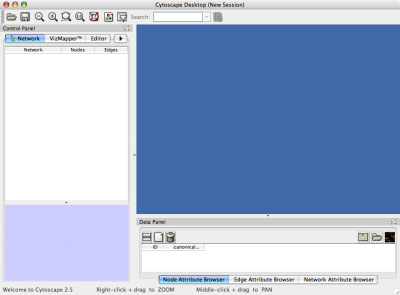
\includegraphics[width=\textwidth]{images/cytoscape_startup_mac.png}
			\caption{Cytoscape启动界面}
			\label{fig:1.1}
		\end{figure}

		\subsubsection{注意内存使用量}

		随着用用户所加载的网络的规模的增加,Cytoscape所需的内存也会增加。内存的使用量取决于网络对象(节点和边)的数量以及属性的数量。表~\ref{table:4}~和~\ref{table:5}是对内存需求量的粗略估计。

		\begin{table}[htbp]
		\centering
		\begin{tabular}{|l|l|}
			\hline
			对象的数量(节点和边) & 建议内存\\
			\hline
			0 -- 70,000 & 512M(默认值)\\
			\hline
			70,000 -- 150,000 & 800M \\
			\hline
		\end{tabular}
		\caption{无视图情况下的建议内存大小}
		\label{table:4}
		\end{table}

		\begin{table}[htbp]
		\centering
		\begin{tabular}{|l|l|}
			\hline
			对象的数量(节点和边) & 建议内存\\
			\hline
			0 -- 20,000 & 512M(默认值)\\
			\hline
			20,000 -- 70,000 & 800M \\
			\hline
			70,000 -- 150,000 & 1G \\
			\hline
		\end{tabular}
		\caption{有视图情况下的建议内存大小}
		\label{table:5}
		\end{table}

		\subsubsection{Cytoscape的整体内存需求}
		可以通过命令行参数增加Cytoscape的内存大小。例如,如果要给Cytoscape分配1G的内存,可以在命令行输入:
		\begin{verbatim}
		java -Xmx1GB -jar cytoscape.jar -p plugins
		\end{verbatim}

		\subsubsection{堆栈尺寸(stact size)}
		这是另一个跟内存分配有关的选项。Cytoscape的部分功能需要较大的堆栈空间(某些操作所需的临时内存,比如Layout)。由于这个堆栈的大小是独立于前面的Xmx值的,所以有时候Layout算法会因为内存不足而失败。为了避免这种情况,可以用-Xss制定更大的堆。如果对大型网络布局时失败,可以尝试下面的命令:
		\begin{verbatim}
		java -Xmx1GB -Xss10M -jar cytoscape.jar -p plugins
		\end{verbatim}
		选项-Xss10M的意思就是将堆的尺寸设置为10MB。在大部分情况下,这能解决由于内存不足导致的Layout问题。

		\begin{figure}[!h]
		\centering
		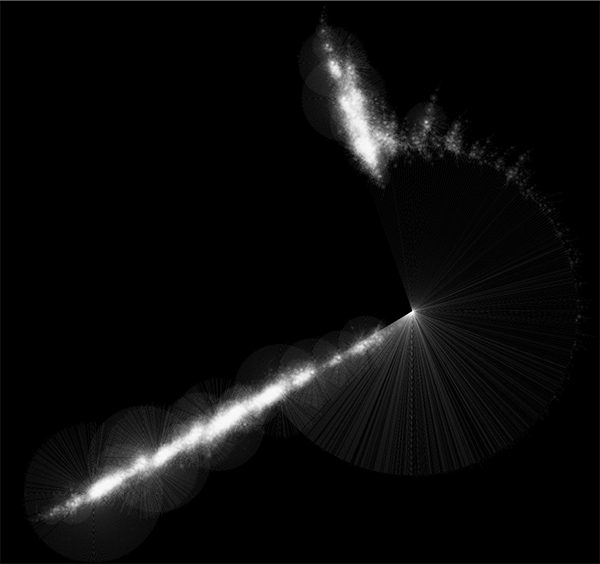
\includegraphics[width=\textwidth]{images/one_million_network.png}
		\caption{\textbf{随机生成的scale-free网络,含有500K个节点和500K条边:}如果正确地设置了内存参数,就能看到这个庞大的网络。在这个例子中,Cytoscape~大约使用了~5GB~内存。堆栈的大小是10MB。如果要使用大内存(大于4GB),就需要64位的操作系统和64位的Java SE 5或6。}
		\end{figure}

		注意:有些web服务客户端是多线程程序,其中没有线程都是使用-Xss选项所指定的内存大小。如果web服务客户端应为内存不足而失败,请调低堆栈的大小,然后再试一次。

		更多的信息请参看\href{How to increase memory for Cytoscape}{http://cytoscape.org/cgi-bin/moin.cgi/How to increase memory 20for Cytoscape}

		\subsubsection{注意目录位置}
		为了能让程序正常运行,在解压后,所有的文件位置都不能随便改动。Cytoscape的核心程序会按照默认的目录结果去查找其所需的库。如果你确实手痒痒想自己改一下,可以通过修改\$CLASSPATH或是cytoscape.jar的manifest文件,这样在任何地方都能启动Cytoscape。
